%https://latex-tutorial.com/latex-appendix/
\appendix
\renewcommand{\thesubsection}{\Roman{subsection}}
\subsection*{Vorlage für einer Fakturierungsalarme in CloudWatch}\label{sec_Ang_A}
JSON\\
\begin{lstlisting}
    "SpendingAlarm": {
 "Type": "AWS::CloudWatch::Alarm",
 "Properties": {
 "AlarmDescription": { "Fn::Join": ["", [
 "Alarm if AWS spending is over $",
 { "Ref": "AlarmThreshold" }
 ]]},
 "Namespace": "AWS/Billing",
 "MetricName": "EstimatedCharges",
 "Dimensions": [{
 "Name": "Currency",
 "Value" : "USD"
 }],
 "Statistic": "Maximum",
 "Period": "21600",
 "EvaluationPeriods": "1",
 "Threshold": { "Ref": "AlarmThreshold" },
 "ComparisonOperator": "GreaterThanThreshold",
 "AlarmActions": [{
 "Ref": "BillingAlarmNotification"
 }],
 "InsufficientDataActions": [{
 "Ref": "BillingAlarmNotification"
 }]
 }
}
\end{lstlisting}

YAML
\\
\begin{lstlisting}
    SpendingAlarm:
    Type: AWS::CloudWatch::Alarm
    Properties:
    AlarmDescription:
    'Fn::Join':
    - ''
    - - Alarm if AWS spending is over $
    - Ref: AlarmThreshold
    Namespace: AWS/Billing
    MetricName: EstimatedCharges
    Dimensions:
    - Name: Currency
    Value: USD
    Statistic: Maximum
    Period: '21600'
    EvaluationPeriods: '1'
    Threshold:
    Ref: "AlarmThreshold"
    ComparisonOperator: GreaterThanThreshold
    AlarmActions:
    - Ref: "BillingAlarmNotification"
    InsufficientDataActions:
    - Ref: "BillingAlarmNotification"
\end{lstlisting}
\footnote{AWS CloudFormation - Benutzerhandbuch. S.481.\cite{AMZ32}}
\newpage

\subsection*{Alarm für die monatliche Kosten anhand eines Budgets}\label{sec_Ang_B}
\begin{figure}[h!]
    \centering
    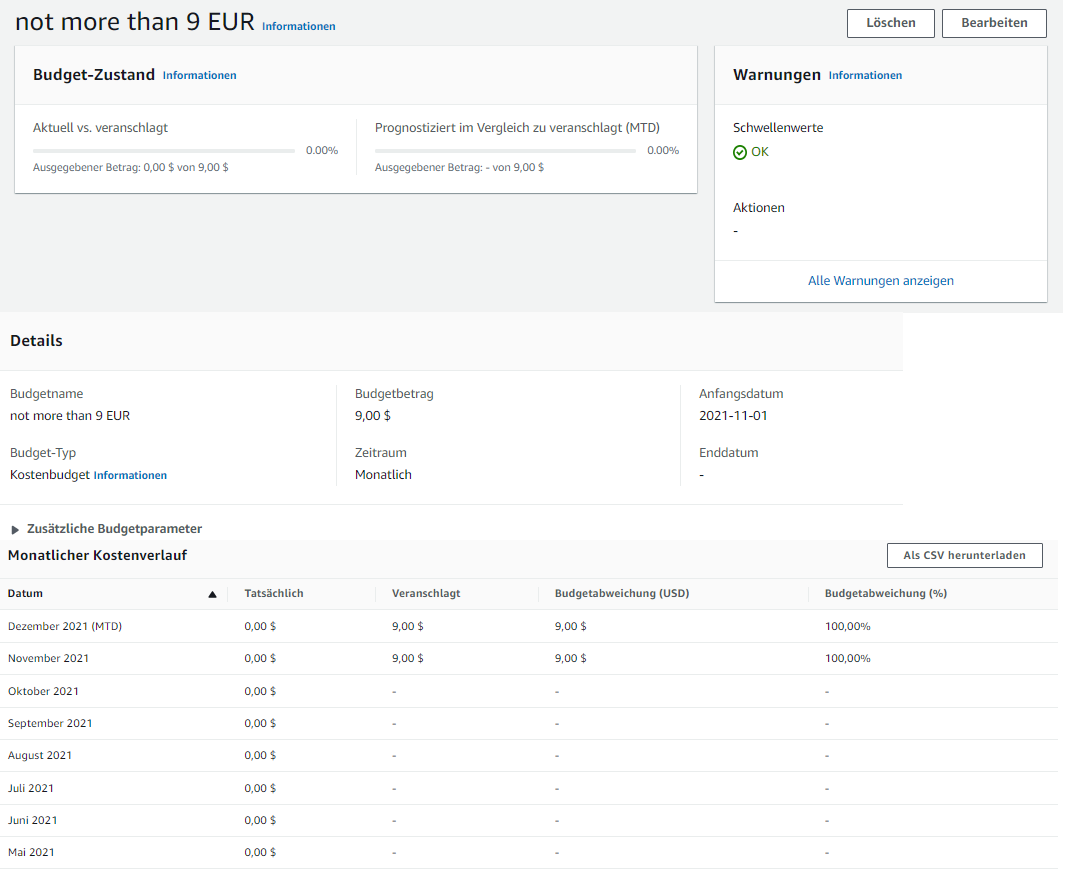
\includegraphics[scale=0.5]{sources/BudgetAlarm}
    \caption[Budgetalarm]{}
    \label{fig:CloudWatchDashboardTest} 
    Eigene Darstellung von Test AWS-Konto.
  \end{figure}
%[Rev Screenshot missing]
%\subsection{Screenshot des CloudWatch-Dashboards}\label{sec_Ang_C}
